\documentclass[10pt]{article}
\usepackage{float}
\usepackage{listings}
\usepackage[french]{babel}
\usepackage[utf8x]{inputenc}
\usepackage{subcaption}
\usepackage{listings}
\usepackage{wrapfig}
\usepackage{color}
\usepackage{amsmath}
\usepackage{dsfont}
\usepackage{amsfonts}
\usepackage{hyperref}
\usepackage{mathtools}
\usepackage{graphicx}
\usepackage{caption}
\definecolor{dkgreen}{rgb}{0,0.6,0}
\definecolor{gray}{rgb}{0.5,0.5,0.5}
\definecolor{mauve}{rgb}{0.58,0,0.82}
\usepackage[table]{xcolor}
\usepackage{adjustbox}
\usepackage{multirow}
%opening
\definecolor{Gray}{gray}{0.85}




\lstset
{frame=tb,
	language=R,
	aboveskip=3mm,
	belowskip=3mm,
	showstringspaces=false,
	framexleftmargin=5mm,
	columns= fixed,
	numbers = left,
	basicstyle={\small\ttfamily},	
	numberstyle=\tiny\color{gray},
	keywordstyle=\color{blue},
	commentstyle=\color{dkgreen},
	stringstyle=\color{mauve},
	breaklines=true,
	breakatwhitespace=true,
	tabsize=3
}


\title{
	\normalfont \normalsize 
	\textsc{Université de Technologie de Compiègne\\ 
		SY09:Analyse des données et Data-Mining , P17} \\
	[10pt] 
	\rule{\linewidth}{0.5pt} \\[6pt] 
	\huge Rendu TP3\\
	\rule{\linewidth}{2pt}  \\[10pt]
}
\author{Zineb Slam, Oumaima Talouka}
\date{\normalsize \today}

\begin{document}
	{\let\newpage\relax\maketitle}	
	
		\begin{abstract}
			Dans ce rapport de TP3 nous allons étudier 2 méthodes d'apprentissage supervisé: le Classifieur Euclidien et les K Plus Proches Voisins. Dans la première partie nous allons implémenter ces 2 méthodes en R. Ensuite nous allons évaluer leur performance avec différents jeux de données. Pour finir, nous allons calculer la règle de Bayes. Les fonctions ayant permis l'obtention de nos résultats sont jointes au rapport du TP.
		\end{abstract}
	
	\section{Classifieur euclidien, K plus proches voisins}
		\subsection{ Programmation}
		Nous avons essayé dans notre implémentation d'éviter les boucles au maximum possible, car celles-ci réduisent les performances.
	La fonction \textit{ceuc.app } retourne les centres d'inertie de chaque classe pour l'ensemble d'apprentissage. La fonction \textit{rowsum} sur R nous a été très utile pour sommer les lignes de chaque classe .\\
	La fonction \textit{ceuc.val}  prédit la classe de chaque individu des données tests. Nous utilisons ici la fonction \textit{distXY} pour calculer la distance qui sépare chaque individu de chaque centre d'inertie.
	
	
		\subsubsection{ Test de fonctions}
		Pour tester nos fonctions nous allons représenter graphiquement les frontières de décision de chaque méthode en appelant les fonctions \textbf{\textit{front.ceuc}} et \textbf{\textit{front.val}} sur les données Synth1-40. On obtient les graphes représentés dans les figures ci-dessous.
			\begin{minipage}{.5\textwidth}
			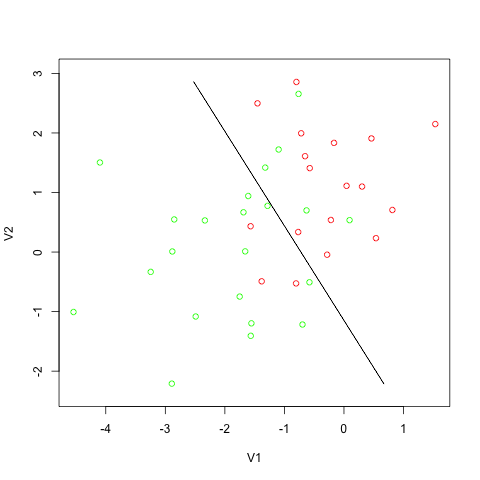
\includegraphics[width=45mm]{Figures/Exo1/front_ceuc.png}
			\captionof{figure}{Frontière de décision obtenue avec le Classifieur Eucledien}
			\label{fig:front_ceuc}
		\end{minipage}%
		\hspace{0.02\linewidth}
		\begin{minipage}{.5\textwidth}
		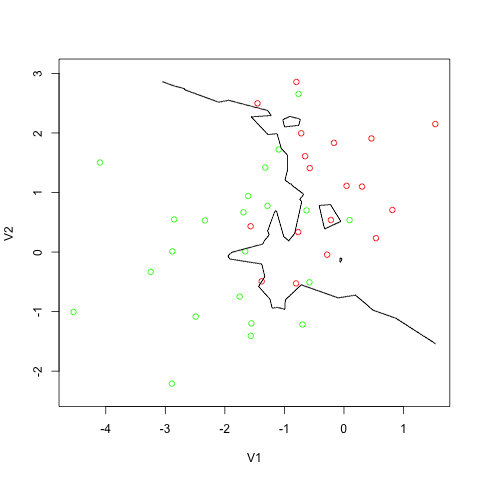
\includegraphics[width=45mm]{Figures/Exo1/front_kppv.png}
			\captionof{figure}{Frontière de décision obtenue avec la méthode des K plus proches voisins (K=3) }
			\label{fig:front_kppv}
		\end{minipage}
		\vspace{0.2mm}
		
		Remarquons que la frontière de décision du classifieur Euclidien est linéaire tandis que celle du KPP est non linéaire.
		
			\subsection{ Évaluation des Performances} \label{section}
			
			\subsubsection{Estimation des paramètres}
			Dans cette partie on estime les moyennes $\mu_{k}$, les matrices de covariances $\Sigma_{k}$ ainsi que les proportions $\pi_{k}$ pour chaque jeu de données et pour chaque classe k. Nous utilisons pour cela 2 fonctions sur R: \textit{group\_by} et \textit{summarize}. La fonction \textit{group\_by} va grouper les données selon les classes z ensuite \textit{summarize} va calculer les paramètres pour chaque groupement. Dans cet exemple on obtient les paramètres de la variable V1.
			\begin{center}		
			\begin{tabular}{ | c | c | c | c | c |}
				\rowcolor{lightgray}
			& &  \multicolumn{3}{c|}{Estimation des Paramètres} \\
			\hline
			 Synth1 & k & $\mu_{k}$ & $\sum_{k}$ & $\pi_{k} $\\
			\hline
			\multirow{2}{*}{40}       &   1&     $\begin{pmatrix} -0.32\\1.09 \end{pmatrix}$                 &     $\begin{bmatrix} 0.68 & 0.12 \\ 0.12 & 1.01 \end{bmatrix}$      & 	0.45				\\\cline{2-5}
			
			      									        &   2&      $\begin{pmatrix} -1.883\\0.105 \end{pmatrix}$          &         $\begin{bmatrix} 1.37 & 0.32 \\ 0.32 &1.44 \end{bmatrix}$        & 			0.55  		\\  
			      									         
			\hline
			\hline
			\multirow{2}{*}{100}      &   1&    $\begin{pmatrix} 0.02\\0.82 \end{pmatrix}$              &           $\begin{bmatrix} 0.88 & -0.13 \\ -0.13 & 1.12 \end{bmatrix}$      & 		0.54	   \\\cline{2-5}
			      											
			      											 &   2&        $\begin{pmatrix} -1.96\\-0.13 \end{pmatrix}$          &         $\begin{bmatrix} 0.76 & -0.04 \\ -0.04 & 0.76 \end{bmatrix}$               & 			0.46		\\
		\hline
		\end{tabular} 
	\end{center}
		\begin{center}		
		\begin{tabular}{ | c | c | c | c | c |}
			\rowcolor{lightgray}
			& &  \multicolumn{3}{c|}{Estimation des Paramètres} \\
			\hline  
			 Synth1 & k & $\mu_{k}$ & $\sum_{k}$ & $\pi_{k} $\\
			\hline   											
			\multirow{2}{*}{500}        &   1&       $\begin{pmatrix} 0.13\\0.88 \end{pmatrix}$            &         	$\begin{bmatrix} 1.05 & 0.052 \\ 0.052 & 0.98 \end{bmatrix}$             & 			0.53		\\\cline{2-5}
			        											&   2&         $\begin{pmatrix} -1.88\\-0.08 \end{pmatrix}$         &  
			        											$\begin{bmatrix} 0.97 & -0.11 \\ -0.11 & 0.98 \end{bmatrix}$                      & 		0.47		\\
		
			\hline
			\hline
			\multirow{2}{*}{1000}         &   1&   $\begin{pmatrix} -0.01\\0.91 \end{pmatrix}$           &        	$\begin{bmatrix} 0.97 & -0.06  \\ -0.06  & 1.08\end{bmatrix}$          & 		0.50		\\\cline{2-5}
			         										&   2&       $\begin{pmatrix} -1.96\\0.02 \end{pmatrix}$            &    $\begin{bmatrix} 0.99 & 0.02 \\0.02 & 0.94 \end{bmatrix}$                  & 	0.50				\\
			\hline
			\end{tabular}
		\end{center}
	
	D'après les résultats du tableau des paramètres de ces jeux de données, nous pouvons remarquer que les matrices $\sum_{k}$ se rapprochent de la forme globale: $\begin{pmatrix} 1 & 0 \\ 0 & 1 \end{pmatrix}$ pour les deux classes, ainsi que des proportions $\pi_{k} $ qui sont quasiment toutes à peu près égales à 0,5. Ainsi, nous pouvons en déduire que les nuages de points sont approximativement sphériques et de même volume. Il est donc possible de séparer les classes par un hyperplan avec le classifieur euclidien.
	
			\subsubsection{Calcul du taux d'erreur du classifieur Euclidien }
			Dans cette partie nous allons tester les performances de chacun des algorithmes programmés précédemment en utilisant le critère de l'erreur qu'on exprime comme:
			\begin{center}
			$Erreur = \frac{1}{N} \sum_{i=1}^{n} {\mathds{1} \hat{z}_{i}  \neq z_{i}}$
			\end{center}
		Avec $z_{i}$ la vrai valeur de z et $\hat{z}_{i}$ la valeur calculée à partir de l'algorithme. N est le nombre d'individus. $\mathds{1} \hat{z}_{i}  \neq z_{i}$ = 1 si $\hat{z}_{i}  = z_{i}$, 0 sinon.
		Après avoir calculé l'erreur qu'on suppose suit une loi normale de moyenne $\mu_{\epsilon}$ et de variance $\sigma_{\epsilon}$, on peut calculer l'intervalle de confiance exprimé ci-dessous.
		\begin{center}
		$Ic = [\mu_\epsilon - t \frac{\sigma_{\epsilon}^2}{\sqrt{N}}, \mu_\epsilon + t \frac{\sigma_{\epsilon}^2}{\sqrt{N}}]$
		\end{center}
	
		On choisit un niveau de confiance t de 95\%. Notons ici que  $\mu$ et $\sigma$ sont ceux calculés pour les différentes valeurs de $\epsilon$ et non ceux du jeu de données. Autre point à remarquer est le N qui est ici le nombre d'individus, or comme on a séparé nos jeux de données en un ensemble d'application et un ensemble de test, on veillera à mettre le nombre d'individus correspondant en fonction si c'est l'intervalle de confiance  d'application ou test. D'après l'énoncé en utilisant la fonction \textit{separ1} napp =$\frac{2n}{3}$  et ntst=$\frac{n}{3}$ n étant le nombre total d'individus du jeu de donnée.
			
			On fait tourner 20 fois le classifieur Euclidien ainsi que le KPP puis on calcule les erreurs obtenus. Les résultats obtenus pour les jeux de données sont affichés dans le tableau qui suit.
			\begin{center}		
				\begin{tabular}{ | c | c| c | c | c |}
						\rowcolor{lightgray} 
				   	&  \multicolumn{4}{|c|}{ Performance du  Classifieur Euclidien}\\
					
					\hline
					 Synth1  &  $\epsilon_{app}$ &  $Ic_{app}$&  $\epsilon_{test}$ &  $Ic_{test}$  \\
					\hline
					\multirow{1}{*}{40}   & 0.23  & $[0.218, 0.234]$& 0.18      & 	$[0.155, 0.205]$ \\
															
					\hline
					\multirow{1}{*}{100}      &0.085  &   $[0.083, 0.088  ]$& 0.102     & 	$[0.093, 0.111]$  \\
				
					\hline
					\multirow{1}{*}{500}     & 0.132 &   $[0.131, 0.132]$& 0.134    & 	$[0.132, 0.136]$	\\
				
					\hline
					\multirow{1}{*}{1000}    & 0.140     & $[0.140, 0.141]$ &  0.147   & $[0.146, 0.147]$  	\\
				
					\hline
				\end{tabular}
			\end{center}
		\vspace{1.5mm}
			En observant les intervalles de confiance, nous remarquons que l'erreur d'apprentissage est inférieure à celle du test, ce qui est normal vu qu'on a entrainé le modèle avec ses données. On remarque aussi que plus le nombre d'individus augmente plus l'intervalle de confiance diminue, ce qui est logique car avec plus de données, le modèle d'apprentissage "apprend" mieux les données et donc pourra mieux classer l'ensemble de test. Notons ici le faible taux d'erreur qu'on a obtenu avec les données \textbf{Synth1-100}, ce qui peut revenir à la génération de données.
			 
				\subsubsection{Le nombre Optimal de voisins du KPP }
				Le nombre optimal de voisins qu'en peut obtenir en ayant l'ensemble d'apprentissage comme ensemble de validation (Xval = Xapp) est toujours de 1 puisque le plus proche voisin d'un individu est lui-même et donc chaque individu sera attribué à sa vraie classe (zval = zapp). L'erreur sera donc nulle dans ce cas et le modèle sera alors biaisé, d'où l'intérêt d'avoir un ensemble d'apprentissage, un ensemble de validation pour déterminer le meilleur k puis un ensemble de test.
			
				\subsubsection{Calcul du taux d'erreur du KPP }
				De la même manière qu'avec le Classifieur Euclidien, nous obtenons les résultats des taux d'erreurs ci-dessous. Notons ici que la notion d'erreur d'apprentissage n'a pas de sens ici car le modèle n'a pas besoin d'apprendre d'abord sur des données puis tester, il fait tout en un seul appel de fonction.
		\begin{center}		
			\begin{tabular}{ | c | c | c |}
				\rowcolor{lightgray} 
				  &  \multicolumn{2}{c}{Performance du KPP}\\
				
				\hline
				Jeu de données Synth1 &   $\epsilon_{test}$ &  $Ic_{test}$\\
				\hline
				\multirow{1}{*}{40}       &0.295  & $[0.253, 0.337]$ 			 \\
				
				\hline
				\multirow{1}{*}{100}      & 0.104 	& $[0.094, 0.114]$  \\
				
				\hline
				\multirow{1}{*}{500}      &  0.152  & 	$[0.149, 0.154]$	\\
				
				\hline
				\multirow{1}{*}{1000}      & 0.146  & 	$[0.144, 0.147]$ 		\\
				
				\hline
			\end{tabular}
		\end{center}
	

			\subsection{Analyse des résultats } 
			 En comparant les 2 méthodes, on remarque que l'erreur ainsi que les intervalles de confiance du Classifieur Euclidien sont bien inférieurs à ceux de la méthode des KPPV. On peut donc conclure que les classes sont linéairement séparables et émettre l'hypothèse que les classes ont les mêmes dispersion et volume.
			
				\subsubsection{ Jeux de données Synth2-1000}
				
					\begin{center}		
					\begin{tabular}{ | c | c | c | c | c |}
						\rowcolor{lightgray} \multicolumn{5}{|c|}{Estimation des Paramètres} \\
						\hline
						Jeu de données & k & $\mu_{k}$ & $\sum_{k}$ & $\pi_{k} $\\
						\hline
						\multirow{2}{*}{Synth2-1000}       &   1&  $ \begin{pmatrix} 3.018\\-0.0063 \end{pmatrix} $             &     $\begin{bmatrix} 0.9904 & 0.1131 \\ 0.1131 & 1.092 \end{bmatrix}$      & 	0.52	     	\\\cline{2-5}
																	&   2&   $\begin{pmatrix} -2.142\\-0.0265 \end{pmatrix}$                 &     $\begin{bmatrix} 4.435 & -0.154 \\ -0.154 & 1.030 \end{bmatrix}$      & 	0.48				\\
						\hline
					
					\end{tabular}
				\end{center}
			
				Grâce à cette estimation, on peut remarquer que \[ \lim \pi_{1} = \lim \pi_{1} = 0.5 \quad \mu_{1} = (3, 0)^{T} 
			\quad \mu_{2} = (-2, 0)^{T} \quad \Sigma_{1} = \begin{bmatrix} 1 & 0 \\ 0 & 1\end{bmatrix} \quad \Sigma_{1} = \begin{bmatrix} 5 & 0 \\ 0& 1\end{bmatrix}\]
				\begin{center}		
				\begin{tabular}{ | c | c | c || c | c |}
						\rowcolor{lightgray} 
			 	 &  \multicolumn{4}{c||}{ Performance du Classifier Euclidien}  \\
					\hline
					Jeu de données &   $\epsilon_{app}$ & $Ic_{app}$ & $\epsilon_{test}$ & $Ic_{test}$\\
					\hline
					\multirow{1}{*}{Synth2-1000}     &         0.061   & $[0.061, 0.062]$		&0.063   &		$[0.062, 0.064]$	 \\
					
					\hline
					
				\end{tabular}
			\end{center}
	
		
		\begin{center}		
			\begin{tabular}{ | c | c | c |}
				\rowcolor{lightgray} 
				&  \multicolumn{2}{|c|}{Performance du KPP}\\
				
				\hline
				Jeu de données &   $\epsilon_{test}$ &  $Ic_{test}$\\
				\hline
				\multirow{1}{*}{Synth2-1000}       &0.062   & $[ 0.061, 0.063]$ 			 \\
				\hline
			\end{tabular}
		\end{center}
				Contrairement aux jeux de données \textit{Synth1-n} on remarque que le KPP semble donner des résultats légèrement meilleurs avec \textit{Synth2}.
				\subsubsection{ Jeux de données réelles: Pima \& Breast Cancer}
				
			
				
				
				\begin{center}		
				\begin{tabular}{ | c | c | c || c | c |}
					\rowcolor{lightgray} 
					&  \multicolumn{4}{c||}{ Performance du Classifier Euclidien}  \\
					\hline
					Jeu de données &   $\epsilon_{app}$ & $Ic_{app}$ & $\epsilon_{test}$ & $Ic_{test}$\\
					\hline
					\multirow{1}{*}{Pima}     &     0.252   & $[0.251, 0.252]$		&0.236     &		$[0.234, 0.238 ]$	 \\
					\hline
					\multirow{1}{*}{Cancer}     &    0.040   & $[0.040, 0.0407]$& 0.039    &		$[0.038, 0.039]$	 \\
					\hline
					
				\end{tabular}
			\end{center}
				
				
					\begin{center}		
					\begin{tabular}{ | c | c | c |}
						\rowcolor{lightgray} 
						&  \multicolumn{2}{|c|}{Performance du KPP}\\
						
						\hline
						Jeu de données &   $\epsilon_{test}$ &  $Ic_{test}$\\
						\hline
						\multirow{1}{*}{Pima}       & 0.248 & $[0.245, 0.250]$ 			 \\
						\hline
							\multirow{1}{*}{Cancer}       &0.040    & $[0.039, 0.042]$ 			 \\
						\hline
					\end{tabular}
				\end{center}
				
				
				
	
	\section{Règle de Bayes}
	\subsection{Loi Marginale}
	La première remarque qu'on peut faire concernant les paramètres des données de Synth1n et Synth2 est que les matrices de variances $\sum_{1}$ et $\sum_{2} $ sont diagonales, donc les covariances COV(V1, V2) =0. Ainsi on peut en déduire que les variables sont indépendantes. Cette remarque va nous être utile dans le calcul de la loi marginale de chaque classe $\omega_{1} $ et $ \omega_{2}$. Ainsi on peut écrire:
	\begin{equation}
	\begin{split}
		f(X^{1}, X^{2}| \omega_{1}) = f(X^{1}|\omega_{1})  f(X^{2}|\omega_{1})\\
		f(X^{1}, X^{2}| \omega_{2}) = f(X^{1}|\omega_{2})  f(X^{2}|\omega_{2})
		\end{split}
		\label{1}
	\end{equation}
	
En utilisant la formule de la densité d'une loi normale on calcule les densités de variables pour chaque classe pour enfin calculer la densité jointe.

\subsubsection{Synth1}
Dans le cas des jeux de données Synth1 nous avons \[\mu{1}= \begin{pmatrix} 0 \\ 1 \end{pmatrix} \quad \mu_{2}= \begin{pmatrix} -2 \\ 0 \end{pmatrix}, \quad  \Sigma = \Sigma_{1} = \Sigma_{2} = \begin{pmatrix} 1 & 0 \\ 0 & 1	\end{pmatrix} \quad et  \quad \pi_{1} = \pi_{2} = 0.5\]


D'après la formule  \refeq{2} on peut alors exprimer les densités comme suit:\\
\begin{equation}
\begin{tabular}{c | c}
	$f_{X^{1}}(x_{1}|\omega_{1}|) = \frac{1}{\sqrt{2\pi}}exp(-\frac{1}{2} x_{1}^{2})$ & 	$f_{X^{1}}(x_{1}|\omega_{2}|) = \frac{1}{\sqrt{2\pi}}exp(-\frac{1}{2} (x_{1}+2)^{2})$\\\\
	$f_{X^{2}}(x_{2}|\omega_{1}|) = \frac{1}{\sqrt{2\pi}}exp(-\frac{1}{2} (x_{2}-1)^{2})$ & 	$f_{X^{2}}(x_{2}|\omega_{2}|) = \frac{1}{\sqrt{2\pi}}exp(-\frac{1}{2} x_{2}^{2})$\\
\end{tabular}
\label{3}
\end{equation}

On obtient ainsi selon \eqref{1} les densités jointes de chacune des classes ci-dessous:
\begin{equation}
\begin{split}
		f_{X^{1}, X^{2}}(x|\omega_{1}) = \frac{1}{2\pi} exp(-\frac{1}{2}(x_{1}^2 + (x_{2}-1)^{2} ))  \\
f_{X^{1}, X^{2}}(x|\omega_{2}) = \frac{1}{2\pi} exp(-\frac{1}{2}(x_{2}^2 + (x_{1}+2)^{2} ))
\end{split}
\label{4}
\end{equation}


\subsubsection{Synth2}
Dans le cas des jeux de données Synth2 nous avons:
\[\mu{1}= \begin{pmatrix} 3 \\ 0 \end{pmatrix} \quad \mu_{2}= \begin{pmatrix} -2 \\ 0 \end{pmatrix}, \quad   \Sigma_{1} = \begin{pmatrix} 1 & 0 \\ 0 & 1	\end{pmatrix}  \quad  \Sigma_{2} = \begin{pmatrix} 5 & 0 \\ 0 & 1	\end{pmatrix}  et  \quad \pi_{1} = \pi_{2} = 0.5\]

Les densités des variables pour chaque classe sont alors:
\begin{equation}
\begin{tabular}{c | c}
$f_{X^{1}}(x_{1}|\omega_{1}|) = \frac{1}{\sqrt{2\pi}}exp(-\frac{1}{2} (x_{1} -3 )^{2})$ & 	$f_{X^{1}}(x_{1}|\omega_{2}|) = \frac{1}{\sqrt{10\pi}}exp(-\frac{1}{10} (x_{1}+2)^{2})$\\\\
$f_{X^{2}}(x_{2}|\omega_{1}|) = \frac{1}{\sqrt{2\pi}}exp(-\frac{1}{2} x_{2}^{2})$ & 	$f_{X^{2}}(x_{2}|\omega_{2}|) = \frac{1}{\sqrt{2\pi}}exp(-\frac{1}{2} x_{2}^{2})$\\
\end{tabular}
\label{5}
\end{equation}

On obtient ainsi selon \eqref{1} les densités jointes de chacune des classes ci-dessous:
\begin{equation}
\begin{split}
f_{X^{1}, X^{2}}(x|\omega_{1}) = \frac{1}{2\pi} exp(-\frac{1}{2}(x_{1}-3)^2 - \frac{1}{2}x_{2}^2       )  \\
f_{X^{1}, X^{2}}(x|\omega_{2}) = \frac{1}{2\pi\sqrt{5}} exp(-\frac{1}{10}(x_{1}+2)^{2}  - \frac{1}{2}x_{2}^{2})
\end{split}
\label{6}
\end{equation}


\subsection{Courbe d'iso-densité}
Une courbes d'iso-densité correspond à la région où la densité est constante.

\subsubsection{Iso-densité de Synth1}
\textbf{Pour la classe $\omega_{1}$} $f(X^{1}, X^{2}|\omega_{1}) = C_{1} \quad avec \quad C_{1} constante$
\begin{equation}
\begin{split}
exp(-\frac{1}{2} (x_{1}-\mu_{1})^{2} - \frac{1}{2}(x_{2} - \mu{1})^{2})  = 2 \pi \sigma_{11}^{2} \sigma_{22}^{2} C_{1}
\\
(x_{1} - \mu_{1})^{2} + (x_{2} - \mu_{1})^{2} = -2ln(2 \pi \sigma_{11}^{2} \sigma_{22}^{2} C_{1})
\\
x_{1}^{2} + (x_{2} - 1)^{2} = -2 ln(2\pi C_{1})
\end{split}
\label{7}
\end{equation}

 L'équation \eqref{5} obtenue est une équation de cercle de centre $\mu_{1} = \begin{pmatrix} 0 \\ 1\end{pmatrix} $ et de rayon $R^{2} = -2 ln(2\pi C_{1})$.\\
 
 \textbf{De même pour la classe $\omega_{2}$} $f(X^{1}, X^{2}|\omega_{2}) = C_{2} \quad avec \quad C_{2} constante$
 \begin{equation}
 \begin{split}
 (x_{1} - \mu_{2})^{2} + (x_{2} - \mu_{2})^{2} = -2ln(2 \pi \sigma_{11}^{2} \sigma_{22}^{2}C_{2}) 
 \\
 (x_{1} + 2)^{2} + x_{2}^{2} = -2ln(2\pi C_{2})
 \label{8}
\end{split}
 \end{equation}
 
 On obtient encore une fois l'équation de cercle de centre $\mu_{2} = \begin{pmatrix} -2 \\ 0\end{pmatrix} $ et de rayon $R^{2} = -2 ln(2\pi C_{2})$.\\


\subsubsection{iso-densité de Synth2}
\textbf{Pour la classe $\omega_{1}$} $f(X^{1}, X^{2}|\omega_{1}) = C_{3} \quad avec \quad C_{3} constante$
\begin{equation}
\begin{split}
exp(-\frac{1}{2} (x_{1}-\mu_{1})^{2} - \frac{1}{2}x_{2}^{2})  = 2 \pi \sigma_{11}^{2} \sigma_{22}^{2} C_{3}
\\
(x_{1} - \mu_{1})^{2} +  x_{2}^{2} = -2ln(2 \pi \sigma_{11}^{2} \sigma_{22}^{2} C_{3})
\\
(x_{1} - 3)^{2} + x_{2}^{2} = -2 ln(2\pi C_{3})
\end{split}
\label{9}
\end{equation}

L'équation obtenue est une équation de cercle de centre $\mu_{1} = \begin{pmatrix} 3 \\ 1\end{pmatrix} $ et de rayon $R^{2} = -2 ln(2\pi C_{2})$.\\

\textbf{De même pour la classe $\omega_{2}$} $f(X^{1}, X^{2}|\omega_{2}) = C_{4} \quad avec \quad C_{4} constante$
\begin{equation}
\begin{split}
exp(-\frac{1}{10} (x_{1}-\mu_{1})^{2} - \frac{1}{2}(x_{2}-\mu_{2})^{2})  = 2\pi\sqrt{5} \pi \sigma_{11}^{2} \sigma_{22}^{2} C_{4}
\\
(x_{1} - \mu_{1})^{2} +  5(x_{2}-\mu_{2})^{2}  = -10ln(2\pi\sqrt{5}  \pi \sigma_{11}^{2} \sigma_{22}^{2} C_{4})
\\
(x_{1} + 2)^{2} + 5x_{2}^{2} = -10ln(10\pi\sqrt{5}\pi C_{4})
\label{10}
\end{split}
\end{equation}

On obtient cette fois-ci l'équation d'une ellipse de centre $\mu_{2} = \begin{pmatrix} -2 & 0\end{pmatrix}^{T}$.

\subsection{Règle de Bayes}
La règle de Bayes s'exprime de la manière:

\[\delta^{*}(x) = \begin{cases} \omega_{1} & si  \quad \Pr(\omega_{1}|x)>  \Pr(\omega_{2}|x) \\
	\omega_{2} & sinon \end{cases}\]
\begin{equation}
\begin{split}
 \iff \delta^{*}(x) = \omega_{1} \quad & si \quad  \frac{f_{X}(x|\omega_{1})}{f_{X}(x)} \pi_{1}> \frac{f_{X}(x|\omega_{2})}{f_{X}(x)}\pi_{2} \\ 
\iff \delta^{*}(x) = \omega_{1} \quad & si \quad  \frac{f_{X}(x|\omega_{1})}{f_{X}|\omega_{2}(x)} > \frac{\pi_{2}}{\pi_{1}} \\ 
\end{split}
\label{9}
\end{equation}
 Dans la suite nous notons $f_1(x) = f_{X}(x|\omega_{1})$ et $f_2(x) = f_{X}(x|\omega_{2})$

\subsubsection{Synth1}
D'après les densités calculées dans \eqref{4} on obtient: \[\frac{f_{1}(x)}{f_{2}(x)} = exp(2x_{1} + x_{2} + \frac{3}{2})\]
On peut donc exprimer l'inéquation \ref{7} de façon linéaire en introduisant le \textit{log} , ainsi on a
\begin{equation}
\begin{split}
2x_{1} + x_{2} > ln\frac{\pi_{2}}{\pi_{1}} - \frac{3}{2}   \quad \frac{\pi_{2}}{\pi_{1}} = 1 \\
x_{2} >  -2x_{1} - \frac{3}{2}
\label{10}
\end{split}
\end{equation}

Ainsi La règle de Bayes attribuera l'individu à la classe 1 si \eqref{10} est vérifiée sinon à la classe 2. Nous obtenons donc une frontière linéaire si les 2 matrices de covariances sont égales. Nous avons représenté cela de manière graphique sur les données Synth1 avec n=40 et n=50 en utilisant ggplot.\\

			\begin{minipage}{.5\textwidth}
	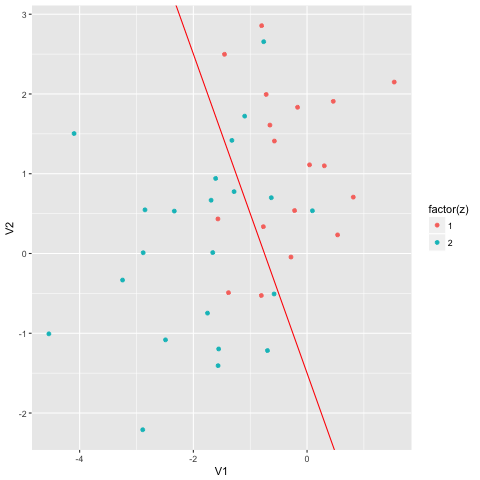
\includegraphics[width=45mm]{Figures/Exo2/linear_synth140.png}
	\captionof{figure}{Frontière de decision Lineaire pour Synth140}
	\label{fig:front_ceuc}
\end{minipage}%
\hspace{0.02\linewidth}
\begin{minipage}{.5\textwidth}
	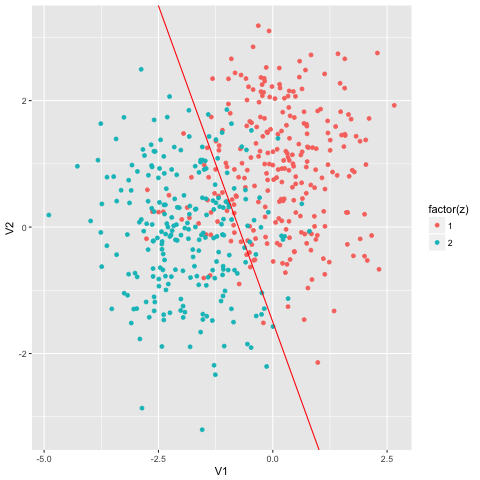
\includegraphics[width=45mm]{Figures/Exo2/linear_synth1500.png}
	\captionof{figure}{Frontière de decision Lineaire pour Synth1500}
	\label{fig:front_kppv}
\end{minipage}

\subsubsection{Synth2}
D'après les densités calculées dans \eqref{4} on obtient: \[\frac{f_{1}(x)}{f_{2}(x)} = \sqrt{5} exp(-\frac{4}{10}x_{1}^{2} + \frac{34}{10} x_{1} - \frac{41}{10})\]

On obtient ainsi l'inéquation: \[-4x_{1}^{2}  + 34x_{1} + 10log\sqrt{5} - 41 > 0\] 
En résolvant cette inéquation de second degré par $\Delta = b^{2} - 4ac$ on obtient 2 solutions
\[k_{2} = 7.197  \quad k_{1} = 1.303 \]

Un individu va donc appartenir à la classe 1 si $k1<x<k2$. Ainsi lorsqu'on a des matrices de covariances différentes on obtient une frontière de décision quadratique. Cette frontière est représentée ci-dessous pour les jeux de données Synth2 en utilisant \textbf{ggplot\textit{}} sur R et stat\_function pour dessiner la courbe.\\

\begin{center}
	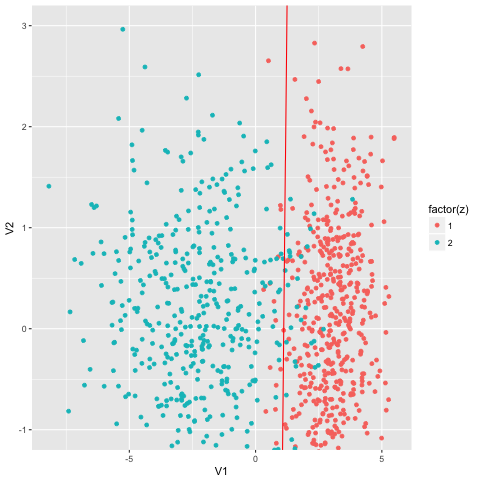
\includegraphics[width=45mm]{Figures/Exo2/curve_synth2.png}
	\captionof{figure}{Frontière de decision Quadratique pour Synth2}
	\label{fig:front1_synth2}
\end{center}%
\hspace{0.02\linewidth}

\vspace{1mm}
Notons qu'on a restreint l'échelle du graphique à celle des données, ce qui fait que la courbe dans la figure \ref{fig:front1_synth2}  n'apparait pas totalement.

\subsection{Erreur de Bayes}
L'erreur de Bayes est la plus petite erreur possible que peut atteindre une règle $\delta$ utilisant uniquement X. 
\subsubsection{Synth1}
Dans le cas des jeux de données de \textit{Synth1n} les matrices de covariances sont égales $(\sigma_{k} = \sigma)$ et les probabilités à priori de chaque classe aussi  ($\pi_{1} = \pi{2}$). Avec ces conditions, l'erreur de Bayes s'écrit sous la forme: \[ \epsilon^{*} = \phi(-\frac{\Delta}{2}) . \]
ou $\phi$ est la fonction de répartition de la loi normale (univariee) centrée réduite  et $ \Delta^{2}   = (\mu_{2} - \mu_{1})^{T} \sigma^{-1} (\mu_{2}  - \mu_{1})$ est la \textit{distance au carrée de Mahalanobis}.\\
On obtient alors $\Delta^{2} = 5$, d'ou $\Delta = \sqrt{5} $ Ainsi: 

\begin{align}
 \epsilon^{*}  &=  \phi(-\frac{\sqrt{5}}{2}) \cr
& =  Pr(x \leq -\frac{\sqrt{5}}{2}) \cr
 &= 1 - \Pr(x \leq \frac{\sqrt{5}}{2})\cr
 & = 1 - 0.86\cr
 \epsilon^{*}  & = 0.13
\end{align}
On remarque  que cette erreur est relativement proche à l'erreur de test $\epsilon_{test}$ du classifieur Euclidien calculée dans la section \ref{section}. 



\subsubsection{Synth2}
Dans le cas général où les matrices de covariances ne sont pas égales, on peut déduire une borne supérieure de l'erreur de Bayes. Dans la page 98 du poly on trouve l'expression de cette borne dans le cas de 2 classes:
\[ \epsilon^{*} \leq \sqrt{\pi_{1}\pi_{2}}  \exp{-\Delta_{B}^{2}} \]
Avec $\Delta_{B}^{2}$ la distance de Bhattacharyya entre les 2 classes et qui s'exprime comme 
\[  \Delta_{B}^{2} = \frac{1}{8} (\mu_{2} - \mu_{1})^{T}  (\frac{\Sigma_{1} + \Sigma_{2}}{2})^{-1} (\mu_{2} - \mu_{1}) + 
\frac{1}{2} ln\frac{|\frac{\Sigma_{1}+\Sigma_{2}}{2}|}{\sqrt{|\Sigma_{1}| |\Sigma_{2}|}} \]

On obtient alors $\Delta_{B}^{2} = \frac{25}{24} +\frac{1}{2} ln(\frac{3}{\sqrt{5}} ) = 1.886$
\[  \epsilon^{*} \leq 0.15\]

Ainsi l'erreur maximale que peut atteindre l'erreur de Bayes est 0.15\\
Maintenant que nous avons une meilleure connaissance de la Règle de Bayes on voudrait connaitre l'erreur commise par cette dernière dans le cas quadratique afin de la comparer à la borne de Bhattacharyya. Ainsi on trouve une faible erreur de l'ordre de 0.056.

\section{Conclusion}
Ce TD nous a permis de se familiariser avec 2 méthodes d'apprentissage supervisé, le classifieur Euclidien et les K Plus Proches Voisins. Ce sont 2 méthodes simples à implémenter mais pas très flexibles, elles sont utiles quand on a peu de données. La règle de Bayes est une méthode de décision qui est intéressante dans le sens où on n'a pas besoin de faire un apprentissage de données et donc moins de temps de calcul. On note ainsi l'importance de connaitre les distributions et les probabilités a priori.
	\end{document}